%Uso da abordagem nos três estudos de dados (Avengers, Aquaman, Capitã Marvel), análise dos resultados e contribuições.

\begin{figure*}[htb]
\begin{center}
% \fbox{\rule{0pt}{2in} \rule{.9\linewidth}{0pt}}
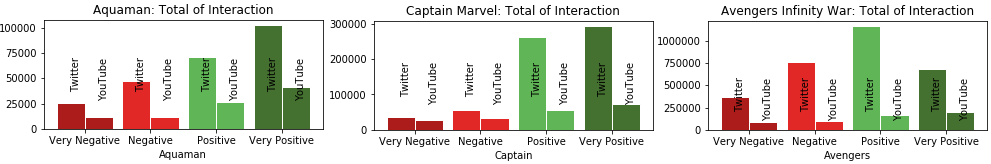
\includegraphics[width=1.0\linewidth]{img/TotalInteractions2.png}
\end{center}
   \caption{Total number of interactions for each movie.}
   % I: acima é preciso especificar porque tem duas barras. Por exemplo: The first bar in each polarity represents the interactions on Twitter and the second on YouTube. 
\label{fig:TotalOfInteractions}
\end{figure*}

%JS: Revisado com o pedro
For the purpose of demonstrating the applicability of our visual analysis approach, we selected three case-studies regarding recently released blockbuster movies to be detailed in the following subsections. We chose these movies in consideration of their popularity in social media, which generated a large volume of data to be analyzed.

\subsection{Dataset Description}

%JS: Mudei o paragrafo abaixo, pois ficou meio repetitivo com o de cima.

%original
%To evaluate the developed approach, we collected data from three major movies releases of the years 2018 and 2019: Avengers Infinite War\footnote{https://www.marvel.com/movies/avengers-infinity-war}, Aquaman\footnote{http://www.aquamanmovie.net/}, and Captain Marvel\footnote{https://www.marvel.com/movies/captain-marvel}. The data gathering process occurred during the debut week of each movie, as showed in Table~\ref{tab:range_data}. 

Our case study data was collected from three major movies releases of the years 2018 and 2019: Avengers Infinite War~\footnote{https://www.marvel.com/movies/avengers-infinity-war}, Aquaman~\footnote{http://www.aquamanmovie.net/}, and Captain Marvel~\footnote{https://www.marvel.com/movies/captain-marvel}. For Twitter, the data gathering process occurred during the debut week of each movie, as showed in Table~\ref{tab:range_data}. For YouTube, we collected all comments available in the official trailers until 03/18/2019, which is the day when the script was executed. 

\begin{table}[h]
    \small{}
    \begin{tabular}{ p{4cm}|p{1.5cm}|p{1.5cm} }
        \hline
            \textbf{Movie} & \textbf{Start} & \textbf{Final}\\
        \hline
            Avengers Infinite War & 04/20/2018  & 05/04/2018 \\
            Aquaman & 12/03/2018 & 12/17/2018  \\
            Captain Marvel & 03/10/2019 & 03/18/2019 \\
        \hline
    \end{tabular}
    \caption{Range of  Twitter data collection.}
    % I: Alterei a legenda acima. A original era: Range of Data Collection. Vejam se concordam.
    \label{tab:range_data}
\end{table}


For data gathering, we used the tools described in Subsection~\ref{sec:datasetCollection}. For Twitter data collection, we used the hashtags: \#AvengersInfinityWar and \#InfinityWar for the Avengers Infinite War movie; \#Aquaman for the Aquaman movie; and \#CaptainMarvel for the Captain Marvel movie. For YouTube, the comments were collected through Marvel's and DC's official YouTube channel\footnote{Infinity War: https://www.youtube.com/watch?v=6ZfuNTqbHE8 and https://www.youtube.com/watch?v=QwievZ1Tx-8}\footnote{Aquaman: https://www.youtube.com/watch?v=WDkg3h8PCVU and https://www.youtube.com/watch?v=fKnL0005qEU}\footnote{Captain Marvel: https://www.youtube.com/watch?v=Z1BCujX3pw8 and https://www.youtube.com/watch?v=0LHxvxdRnYc}.

Our final dataset was distributed as follows: 2.985.563 tweets and 553.618 YouTube comments for Avengers Infinite War; 246.344 tweets and 91.634 YouTube comments for Aquaman; and 650.730 tweets and 189.972 YouTube comments for Captain Marvel. 



\subsection{Results Analysis}

% I: reescrevi o parágrafo abaixo, original em comentário.
The first visualization developed was the bar chart presented in Figure \ref{fig:TotalOfInteractions}. This chart provides an overview of the total and the polarity of tweets in each dataset. It is possible to notice that the Avengers movie was, by far, the most commented movie from the selected 3. It is also possible to see that, even though the collection period is longer on YouTube, most comments were made on Twitter.

Another aspect that can be noticed on this chart is that the proportion between the number of comments in each polarity does not remain the same on YouTube and Twitter. For instance, the number of very negative and negative comments on YouTube remains almost the same for all analyzed movies, but there are significant differences for it on Twitter.
% I: não sei se dá para fazer a afirmação acima... Teria que ver em percentual, não em número absoluto. Mas, deixa isso para o final, só se der tempo.

% I: abaixo não faltou especificar para qual filme no primeiro aspecto? Não seria: The first one was that the number of positive comments overcomes the number of very positives just for Avengers.?
Two other aspects of these charts surprised us. The first one was that the number of positive comments overcomes the number of very positives. The second one was that Captain Marvel had the least amount of negative comments from the overall group. 
The second visualization we developed was the word clouds presented in the Figures~\ref{fig:wordcloudsAquaman}, \ref{fig:wordcloudsCaptain} and \ref{fig:wordcloudsAvengers}. These word clouds provided some meaningful insights about our data. For instance, we can have an idea of which characters will appear on the heatmaps chart. In the word cloud of the movie Avengers, it is possible to notice that the character ''Thanos'' appears on both positive and negative word clouds, and checking the heatmaps, we can verify that he is one of the most mentioned ones.
% I: alterei um pouco o final do parágrafo acima. Original abaixo. Mas, na fig. 6, eu não vi o Thanos nas word clouds positivas, pelo menos não tão grande como nas negativas. Ou estou enganada? Então não seria o caso de dizer que ele aparece nas negativas por ser o vilão da história?
%It is possible to notice that the character ``Thanos'' appears on both positive and negative word clouds, checking the heatmaps, we can verify that he is one of the most mentioned ones.

% I: uma curiosidade é porque o Thanos aparece nas word cloud negativa da capitã Marvel? Talvez possa se dizer que são feitas comparações entre eles, de quem é o mais poderoso. Mas, para isso, teria que pegar alguns tweets de exemplo para justificar a afirmação. Outra curiosidade é porque aparece "panther" na word cloud do filme do Aquaman, se eles são de universo diferentes? De novo, teria que pegar tweets que tenham panther para ver o que dizem...

% I: o que é CGI abaixo? Esta sigla não foi usada antes.
Also, the majority of words used to generate the ``recommendation text'' can be seen in the word clouds. For instance, words like good and best can be seen on the positive word clouds for the Avengers movie, and CGI (computer-generated imagery) can be seen on the negative YouTube word cloud for Aquaman.

Analyzing the word clouds as a whole, we can notice several differences between the Twitter version and the YouTube one. The YouTube word clouds focus more on expectation and technical aspects of the movie, while the Twitter one focus more on viewers' opinions.

% I: abaixo já é sobre o heat map? É que o parágrafo está começando de forma genérica  (The visualization we provided...).
The visualization we provided, shows which ones are the most commented characters of a movie, and the most common words used to describe it. In the same way as the word cloud visualization, we can notice that the words used in YouTube are different from the ones used on Twitter. Regarding the characters, they remain relatively the same on both social media, with some minor differences.

Also, for the characters is possible to notice that, if a character has a high number of interaction in one social media, it is most likely to have a high number of communications on the other ones. This statement is also valid for the heatmap polarity. If a character was highly commended in the positive heatmap, it probably will, also, appear on the negative heatmap. There are a few exceptions for this statement like, for instance, the Black Widow character on Twitter and Korath character on YouTube.

\begin{figure*}[htb]
\begin{center}
    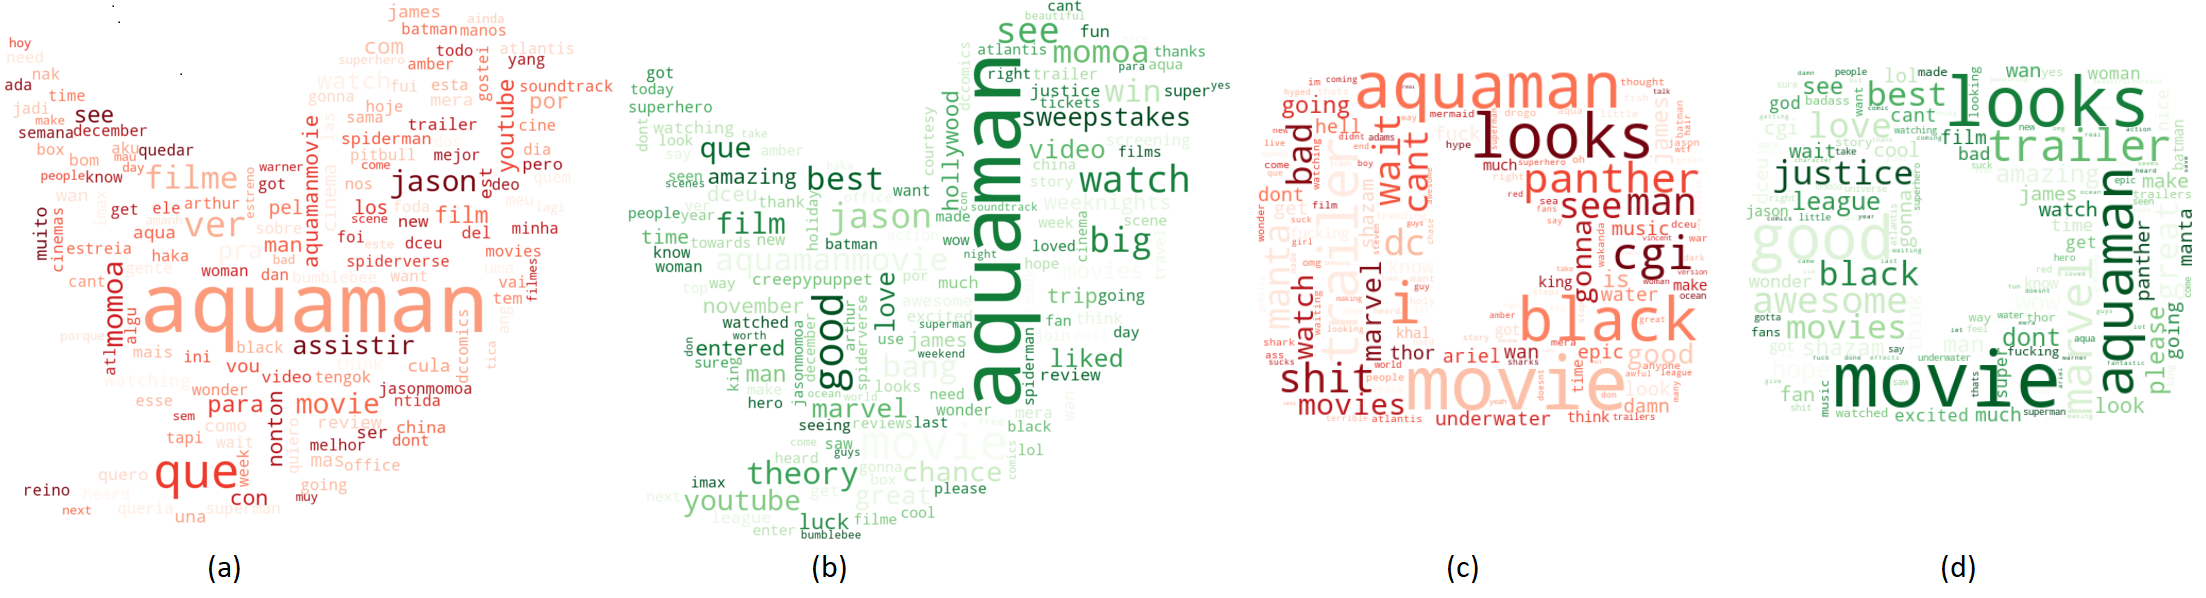
\includegraphics[width=1\linewidth]{img/wordcloudsAquaman.png}
\end{center}
  \caption{Positive (green) and negative (red) word clouds with most used terms in Tweets (a,b) and YouTube comments (b,c) about Aquaman movie.}
  % I: quem sabe alterar a legenda acima para:
  % Positive (green) and negative (red) word cloud with most used terms in Tweets (a,b) and YouTube comments (b,c) about Aquaman movie.
  % Se concordarem, usar o mesmo "padrão" nas demais. 
\label{fig:wordcloudsAquaman}
\end{figure*}

\begin{figure*}[htb]
\begin{center}
    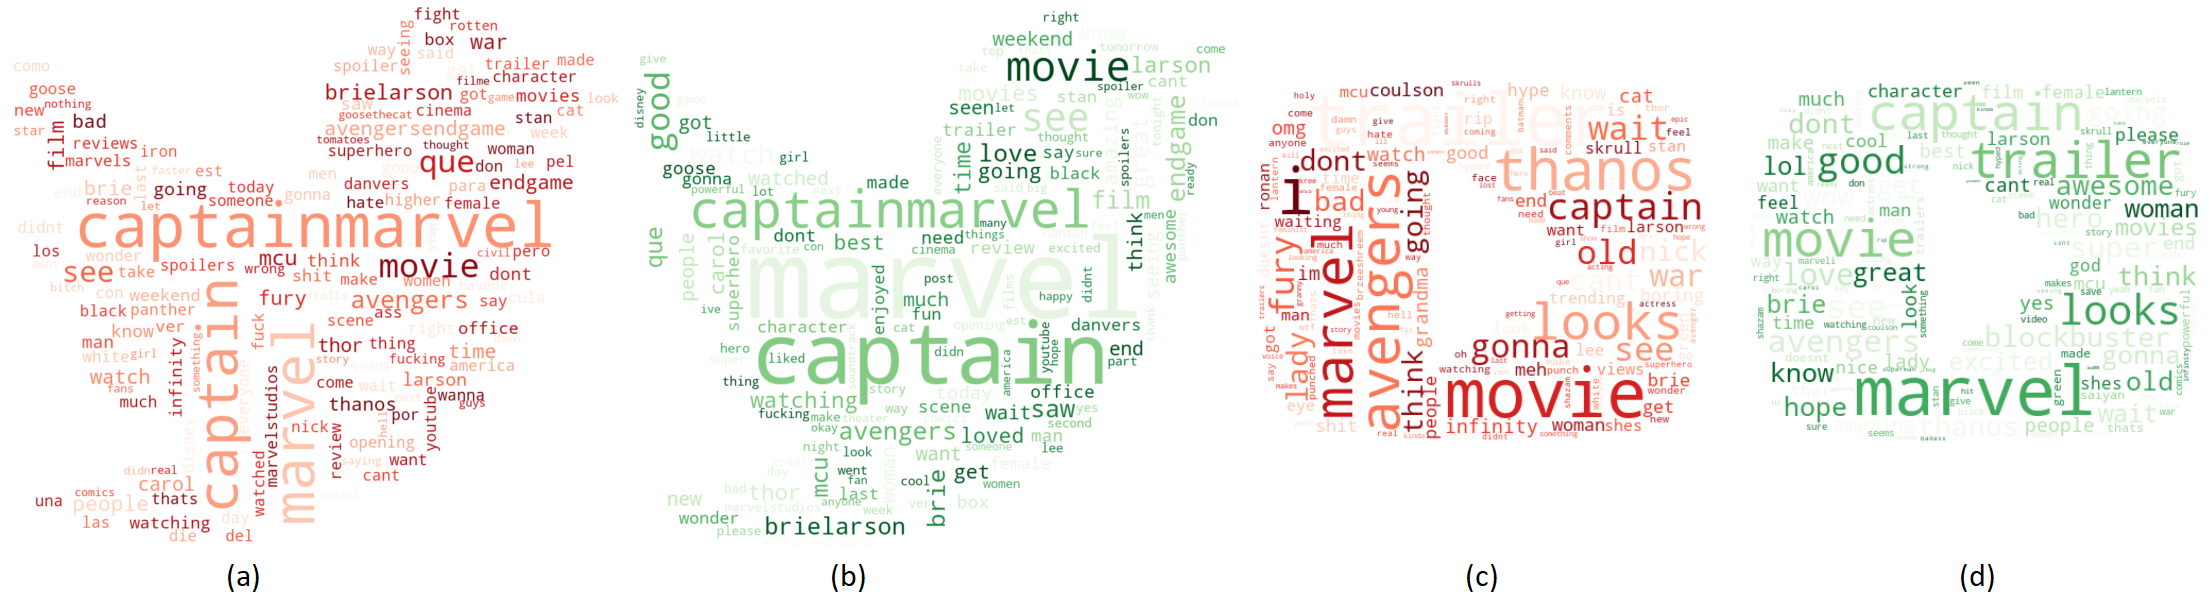
\includegraphics[width=1\linewidth]{img/wordcloudsCaptain.png}
\end{center}
  \caption{Positive (green) and negative (red) word clouds with most used terms in Tweets (a,b) and YouTube comments (b,c) about Captain Marvel movie.}
\label{fig:wordcloudsCaptain}
\end{figure*}

\begin{figure*}[htb]
\begin{center}
    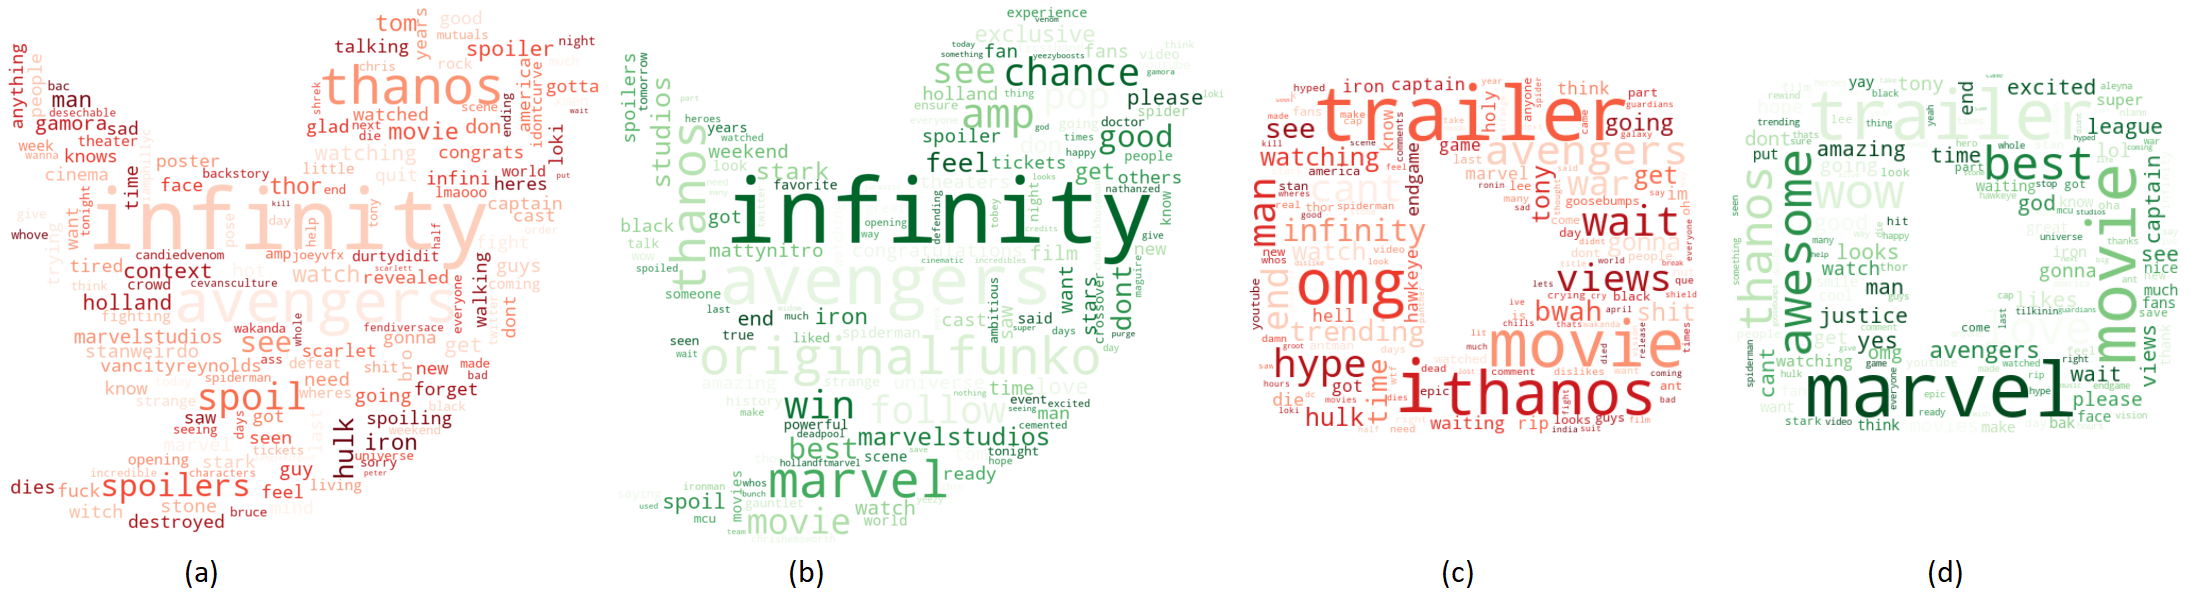
\includegraphics[width=1\linewidth]{img/wordcloudsAvengers.png}
\end{center}
  \caption{Positive (green) and negative (red) word clouds with most used terms in Tweets (a,b) and YouTube comments (b,c) about Avengers Infinity War movie.}
\label{fig:wordcloudsAvengers}
\end{figure*}

%
\begin{figure*}[htb]
\begin{center}
    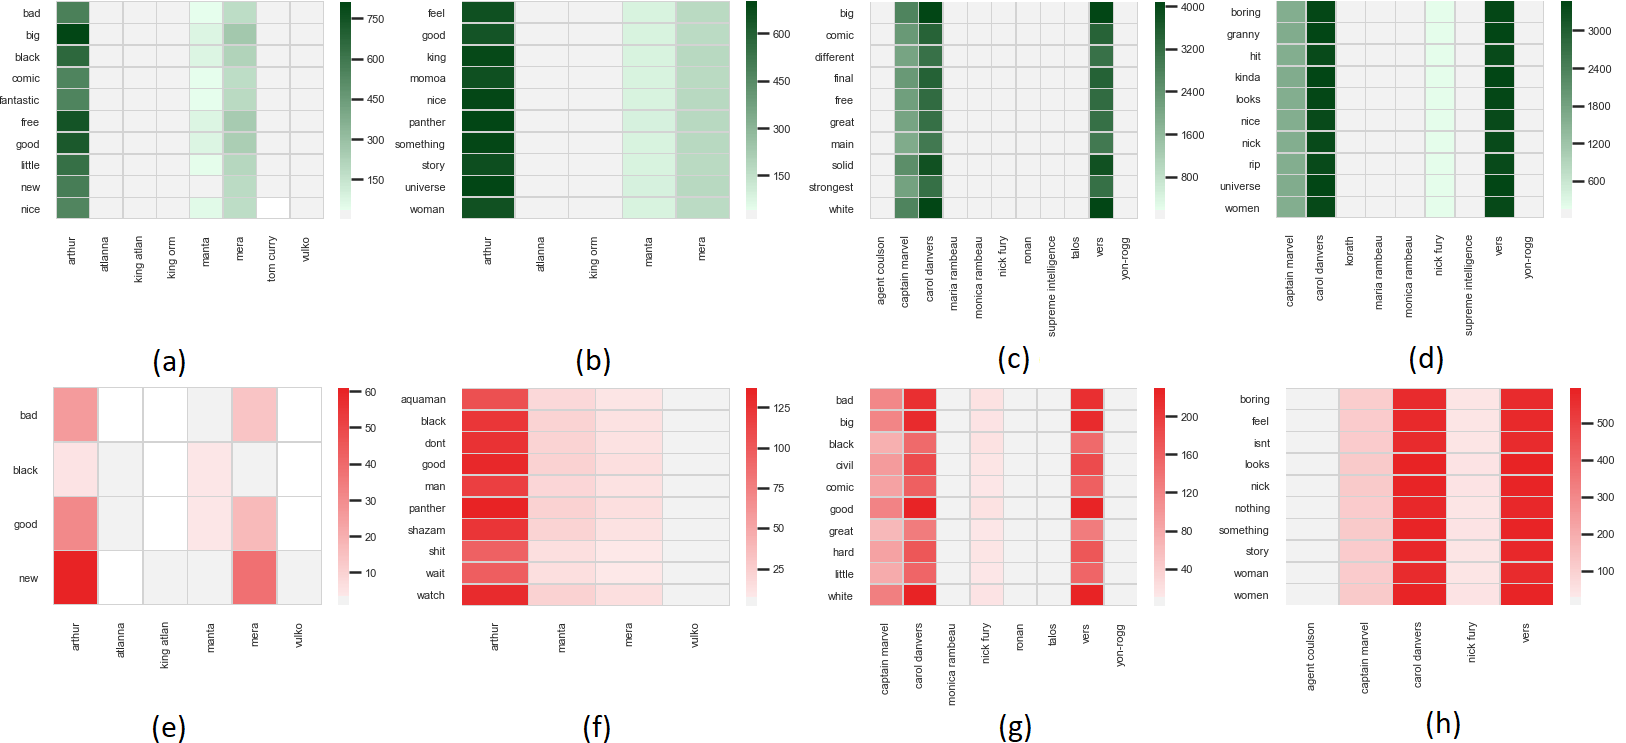
\includegraphics[width=1\linewidth]{img/AquamanCapitaHeatMap.png}
\end{center}
   \caption{Positive (green) and negative (red) heatmaps with the top 10 most used words to describe character in Tweets and YouTube comments. Twitter positive heatmap for Aquaman (a); YouTube positive heatmap for Aquaman (b); Twitter positive heatmap for Captain Marvel (c); YouTube positive heatmap for Captain Marvel (d);
   Twitter negative heatmap for Aquaman (e); YouTube negative heatmap for Aquaman (f); Twitter negative heatmap for Captain Marvel (g). YouTube negative heatmap for Captain Marvel (h).}
   % I: Quando arrumar esta legenda, especificar cada letra.
\label{fig:AquamanCapitaHeatMap}
\end{figure*}

\begin{figure*}[htb]
\begin{center}
    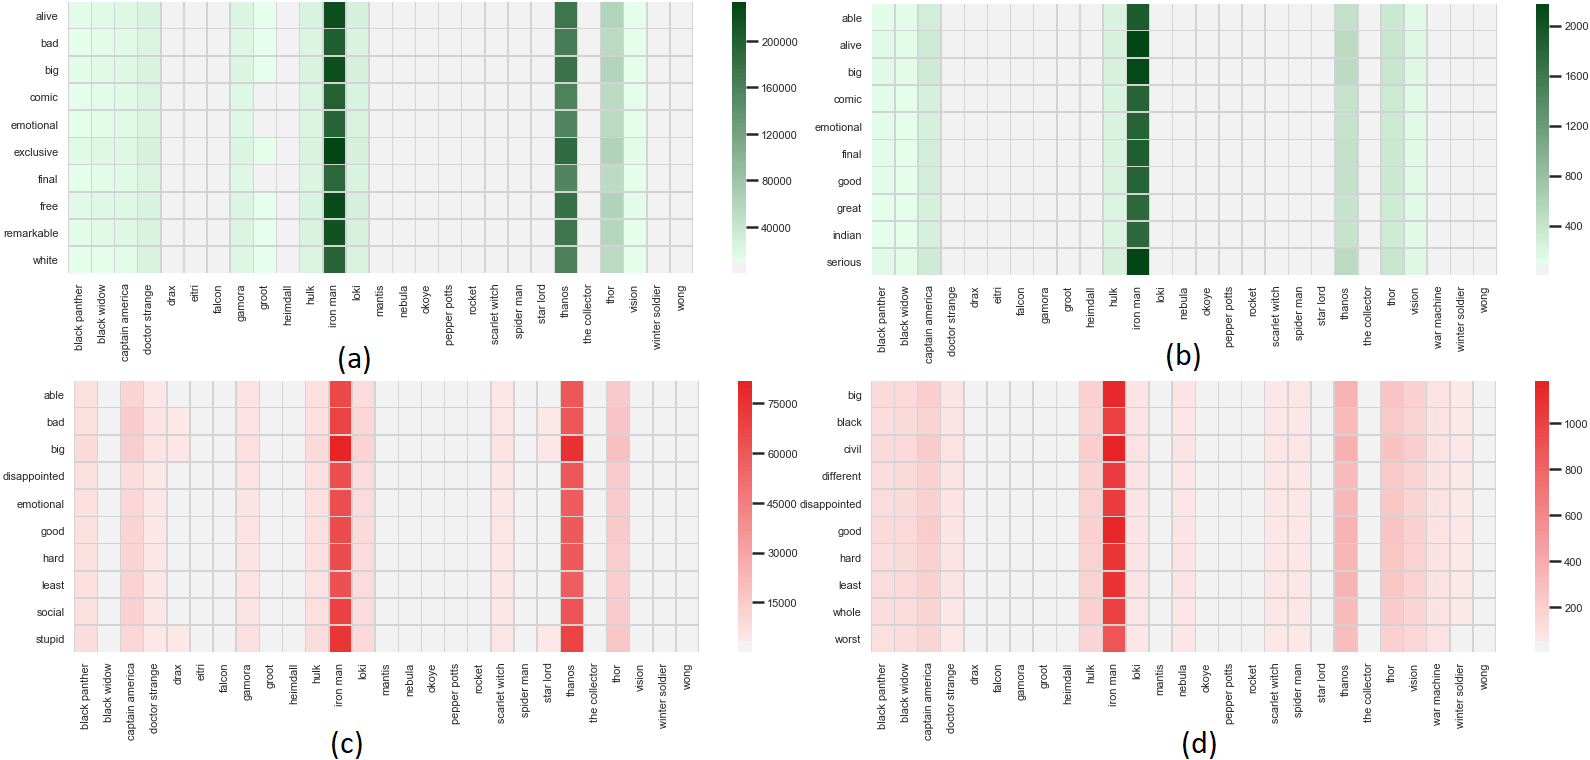
\includegraphics[width=1\linewidth]{img/VingadoresHeatMap.png}
\end{center}
   \caption{Positive (green) and negative (red) heatmaps with the top 10 most used words to describe character in Tweets and YouTube comments. Twitter positive heatmap (a); YouTube positive heatmap (b); Twitter positive heatmap (c); YouTube positive heatmap (d) for Avengers Infinity War.}
\label{fig:VingadoresHeatMap}
\end{figure*}

\subsection{Textual recommendation and Word Clouds}

%In this step, we use the TF-IDF features to evaluate how important is a certain term/word in a given document~\cite{Dipanjan:2016}. From the results obtained by the lexicons, we divided in files, according with texts polarity, to calculate the TF-IDF. Therefore, we will have the most used terms in negative and positive texts.

% In this step, we use the TF-IDF features to evaluate how important a certain term/word is in a given document~\cite{Dipanjan:2016}. The results obtained by the sentiment analysis with Vader, were divided into files, according to the polarity defined by the lexicon in each text, and then the TF-IDF was applied. Therefore, we will have the most used terms in negative and positive texts.

%In this step, we used TF-IDF features to evaluate how important a certain term/word is in a given document. The results obtained by the lexicons were divided into files, according to their polarity, and then the TF-IDF was applied. Therefore, we will have the most used terms in negative and positive texts. 
%SO: aqui acima... no passo a passo ainda não sabemos se é positivo ou neg no paragrafo acima né? achei essa section mal explicada e confusa

% From the most used terms found in the texts, we proceed to the identification the lexical category in which the words are assigned based on their syntactic context and role, called POS (Part-of-Speech) Tagging. Using NLTK Library, which generates outputs specific tags for certain word, we could find: \textit{Adjectives, Nouns, Adverbs, Coordination Conjunction, Verbs, Preposition and etc}, as showed in Listing \ref{tfidf}. 

%SO: ao invés deste "can mention", que tal "could find"



Manually, we created text recommendations about analyzed movies, based on the terms generated by TF-IDF, respecting the text's syntatic structure. The Text Recommendation is presented in Table~\ref{ref:text-rec}.  

\begin{table}[h!]    
    \small
    \begin{tabular}{  l | p{6cm} }
    \hline
        \textbf{Movie} & \textbf{Text Recommendation} \\ 
    \hline
        \multirow{6}{*}{\textbf{Avengers}} & \textbf{Pos:} Avengers was \textit{greatest, biggest, best} movie I had seen. With \textit{huge} and \textit{fantastic} fight scenes, and \textit{hilarious} dialogues between the characters. \textbf{Neg:} Avengers made me \textit{angry, depressed, worried, and physically weak} with the final scene. \\ 
    \hline
        \multirow{6}{*}{\textbf{Aquaman}} & \textbf{Pos:} Aquaman \textit{impressed} (\textit{surprised}) me \textit{positively}, with \textit{incredibles} visual effects. DC Comics has built a great, fantastic and solid movie for all fans. \textbf{Neg:} Aquaman has \textit{missing cgi} in some scenes, in addition to \textit{exploring} little \textit{fight} scenes. \\ 
    \hline
        \multirow{8}{*}{\textbf{Captain M.}} & \textbf{Pos:} Captain Marvel proved \textit{strong, powerful} and \textit{ready} for any battle. Marvel delivered an \textit{important character}, capable of impressing the \textit{capable impressing audience} that didn't know it. \textbf{Neg:} The movie \textit{reminds} me \textit{Green Lantern}. And the way she got your \textit{powers}, wasn't well \textit{solved} in the movie.\\
    \hline
    \end{tabular}
    \caption{Text Recommendation about movies.}
    \label{ref:text-rec}
\end{table}

In addition, we present Word Clouds based on results from TF-IDF. The corpus of these Word Clouds is about texts extracted from tweets during week premiere, and trailers comments on YouTube. It contains all the main terms, organized by color, red for negative and very negative terms, green for positive and very positive, by mask according to the social network, and by movie, as shown in Figures \ref{fig:wordcloudsAquaman}, \ref{fig:wordcloudsCaptain}, \ref{fig:wordcloudsAvengers}.

% \subsection{HeatMap}

% The Heat Map build, aims to show the degree most used terms occurrences in relation to the main characters of each movie. This process is composed of 4 phases. The first phase, is to collect the list of main characters in each movie. Then, we search for each character in the list, in the set of already classified texts, and store the texts that have this condition in a temporary list. 

% The third phase, we try to find in the resulting TF-IDF files, the terms classified as \textit{Adjectives} and that have at least 100 appearances in texts, and we also save in a temporary list. The last phase, is concerned with run the temporary list of text generated in phase 2, in the search for terms established in the phase 3. If condition is true, we add in a incremental variable, the number of times a given term is mentioned for each character. 

%SO: acima nos resultados... aquele texto a direita pe de alguem especifico? ou gerado?

